% Chapter 2

\chapter{Fundamentação Teórica}\label{chap:background}


\section{Área dos Negócios}\label{sec:business}


\section{Fundamentos da Área}\label{sec:fundamental}

Equação ~\ref{eq:my_equation} é um exemplo de uma equação em Latex:


\begin{equation}\label{eq:my_equation}
    h_t = f(W^{(hh)}h_{t-1} + W^{(hx)}x_t).
\end{equation}


Figura\ref{fig:diagram} é um exemplo para incluir uma figura.

\begin{figure}[htb]
    \caption{Simple diagram}
    \centering
    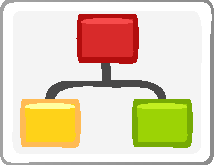
\includegraphics[scale=1.9]{img/diagram.pdf}
    \label{fig:diagram}
    \source{Retirado de \cite{larcc}.}
\end{figure}

\cite{GRIEBLER:IJPP:18}


\cite{MACCOOL:structured_patterns:book:12}


\section{Trabalhos Relacionados}\label{sec:rw}

São apresentados neste tópico, os trabalhos relacionados, que possuem
algum ponto em comum com o que se quer realizar no presente projeto.
Pretendesse aqui, identificar estes pontos, e compará-los com a proposta deste projeto.

\subsection{BDTC - Uma Biblioteca Digital de Trabalhos Científicos com Serviços Integrados}

O trabalho desenvolvido por \cite{CERVI:bdtc}, possui como premissa a apresentação
de uma proposta de biblioteca digital de trabalhos científicos, que foi denominada como
BDTC, que possui como objetivo prover o suporte a três pontos fundamentais:
auto-arquivamento do conteúdo, extração de metadados e busca de similaridade.

Como um dos principais diferenciais, foi desenvolvido um mecanismo de
busca por similaridade para as pesquisas realizadas na BDTC,
que permite ao usuário encontrar trabalhos relacionados, mesmo que
parte da palavra pesquisada não seja exatamente igual ao conteúdo presente
no documento.

Para o desenvolvimento deste mecanismo de busca, foi utilizado
um recurso denominado \emph{n-gram}, que permite quebrar uma palavra em
conjuntos de letras de tamanhos variados, é retratado como exemplo o
\emph{3-gram} do termo "Juci", que pode ser quebrado em dois conjuntos de 3
letras, ou seja, \emph{"Juc"} e \emph{"uci"}.

Estes conjuntos são armazenados em uma tabela de indices no banco de
dados, de forma que ao realizar uma consulta a partir de uma palavra,
o sistema retorna todos os trabalhos que contenham algum dos conjuntos
de letras que compõem a palavra pesquisada.

Em relação com o presente projeto, pode ser realizado uma comparação com
a forma como o mecanismo de busca foi desenvolvido na BDTC. Ao envés de
utilizar o recurso de \emph{n-gram}, o sistema proposto neste projeto utilizara
o recurso de \emph{tokenization} presente na ferramenta de Full Text Search do
banco de dados PostgreSQL, que possui um resultado final semelhante, porem não
idêntico, visto que o \emph{tokenization} remove o gênero das palavras,
os espaços em branco, palavras comuns e palavras que não são consideradas relevantes.

\subsection{Desenvolvimento da nova Biblioteca Digital da Biblioteca Brasiliana USP: Relato de Experiência}

O relato de experiência desenvolvido por \cite{GarciaRodrigoMoreira2019DdnB}
apresenta o desenvolvimento da na nova plataforma de Biblioteca Digital da
BBM, a Biblioteca Brasiliana Guita e José Mindlin, em forma de retrospectiva
desde o projeto-piloto, relatando os principais problemas, êxitos
e desafios encontrados durante o desenvolvimento do projeto, que envolvia
a digitalização e desenvolvimento de uma coleção digital para a biblioteca.

A Biblioteca Brasiliana Guita e José Mindlin foi inaugurada em março
de 2013, sendo um órgão e entidade acadêmica da Pró-Reitoria de Cultura
e Extensão da USP (Universidade de São Paulo). Este biblioteca envolve o
projeto Brasiliana USP, que foi iniciado em 2005, e tem como objetivo
abrigar a coleção Brasiliana, doada por José Mindlin. Dentro do escopo
deste projeto, em 2008 é iniciado o projeto-piloto da Biblioteca
Brasiliana Digital, que visa a preservação do acervo e democratização
do acesso ao material.

Para o desenvolvimento da biblioteca digital, foi optado por realizar uma
customização do sistema DSpace, um software open source de repositório
digital, com recursos como o Djatoka (servidor de imagens) e visualizadores
de livros como IIPImage e BookReader.

Como principais problemas e êxitos, foi ressaltado a forma como as customizações
foram realizadas no DSpace, sendo muitas delas realizadas diretamente no código fonte
do programa, tornando extramente difícil ou até impossibilitando a atualização
para novas versões da plataforma. Resultado em inconsistências na
visualização dos documentos digitalizados, lentidão do sistema, dentro outros
problemas que vieram a surgir ao longo do tempo.

Além disto, também foi relatado a rotativada das equipes como um fator de impacto
para a continuidade do desenvolvimento da biblioteca, que em sua
maioria era constituída por bolsistas, estagiários e poucos profissionais
terceirizados contratados por tempo determinado. Também foi constatado
que as máquinas digitalizadoras adquiridas para a biblioteca não eram
adequadas para o manuseio dos documentos do acervo, visto que os documentos
eram obras raras, e que necessitavam de diversos cuidados para a preservação
e conversação do material.

Com o tempo parte dos problemas foram resolvidos, sendo até adquirido novas
maquinas digitalizadoras, mais modernas e adequadas para o manuseio do material
bibliográfico.

Comparando o trabalho relacionado com o presente projeto de pesquisa,
é possível ressaltar que o atual projeto não tem como intenção a digitalização
de um acervo físico, porem o sistema DSpace que foi utilizado no trabalho
relacionado foi identificado como um sistema muito popular para o desenvolvimento
de repositórios acadêmicos e bibliotecas digitais de universidades, sendo
possível utilizar a experiência adquirida na implantação desse sistema durante
o desenvolvimento do repositório acadêmico proposto.

\subsection{Classificação facetada: proposta de categorias fundamentais para organizar teses e dissertações em uma biblioteca digital}

